\documentclass[border=10pt]{standalone}
\usepackage{tikz}\usepackage{amsmath}\usetikzlibrary{calc,arrows.meta}
\begin{document}
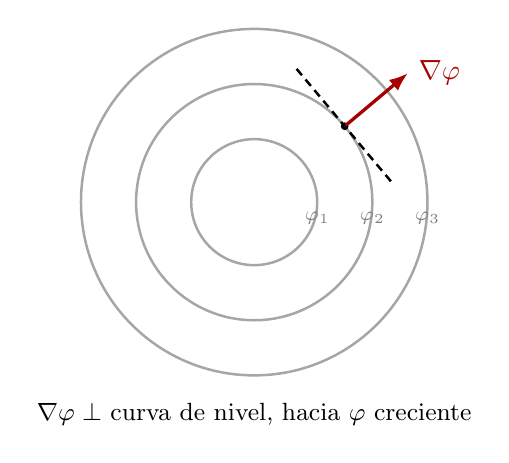
\begin{tikzpicture}[line width=0.9pt,>={Latex[length=2.4mm]}]
  \foreach \r/\v in {0.8/1,1.5/2,2.2/3} {\draw[gray!70] (0,0) circle(\r);}
  \node[gray] at (0.8,0)[below]{\scriptsize $\varphi_1$};
  \node[gray] at (1.5,0)[below]{\scriptsize $\varphi_2$};
  \node[gray] at (2.2,0)[below]{\scriptsize $\varphi_3$};
  \coordinate (P) at (40:1.5);
  \fill (P) circle(1.4pt);
  \draw[->,red!65!black,line width=1.2pt] (P)--($(P)+(40:1.05)$) node[right]{$\nabla\varphi$};
  \draw[densely dashed] ($(P)+(130:0.95)$)--($(P)+(310:0.95)$);
  \node at (0,-2.7){\small $\nabla\varphi\perp$ curva de nivel, hacia $\varphi$ creciente};
\end{tikzpicture}
\end{document}
